\section{Задача № 2}

Дано векторное поле \(\vec{H} : \left( e^x, -e^y \right)\).

\begin{enumerate}
  \item Убедитесь, что данное векторное поле потенциально.
  \item Найдите уравнения векторных линий. Изобразите векторные линии на
        рисунке.
  \item Найдите потенциал поля при помощи криволинейного интеграла.
  \item Найдите уравнения линий уровня потенциала (эквипотенциальных линий).
        Изобразите линии уровня потенциала.
  \item Докажите ортогональность найденных векторных линий поля и линий уровня
        потенциала. Проиллюстрируйте ортогональность на графике.
  \item Выберите какую-либо векторную линию поля и зафиксируйте на ней точки
        \(A\) и \(B\), выбрав для них числовые координаты. Вычислите работу поля
        вдоль этой линии, используя найденный в п. 3) потенциал.
\end{enumerate}

\subsection{Решение}

Обозначим \(\vec{H} = P(x, y) \vec{i} + Q(x, y) \vec{j}\), где
\(P(x, y) = e^x\), \(Q(x, y ) = -e^y\).

Поле будет потенциальным, если найдется функция \(\Phi(x, y)\) (называемая
потенциалом) такая, что её частные производные по \(x\) и \(y\) будут равны
\(P(x, y)\,dx\) и \(Q(x, y)\,dy\) соответственно.

Рассмотрим функцию \(\Phi(x, y) = e^x - e^y\), вычислим её частные производные:

\begin{equation*}\begin{split}
    \Phi'_x = e^x\,dx \\
    \Phi'_y = -e^y\,dy
  \end{split}\end{equation*}

Получаем, что \(\Phi'_x = P(x, y)\,dx\) и \(\Phi'_y = Q(x, y)\,dy\), значит
функция \(\Phi(x, y)\) является потенциалом этого поля, а значит поле является
потенциальным.

\bigskip

Найдем уравнения векторных линий, для этого решим дифференциальное уравнение
\(Q(x, y)\,dx = P(x, y)\,dy\):

\begin{equation*}\begin{split}
    -e^y\,dx = e^x\,dy \\
    \int -e^{-x}\,dx = \int e^{-y}\,dy \\
    e^{-x} = -e^{-y} + A \hspace{3pt} (A > 0, A \in \mathbb{R})\\
    e^{-x} + e^{-y} = A
  \end{split}\end{equation*}

Получили уравнение для векторных линий \(e^{-x} + e^{-y} = A\).

Изобразим на графике некоторые из них при разных значениях \(A\).

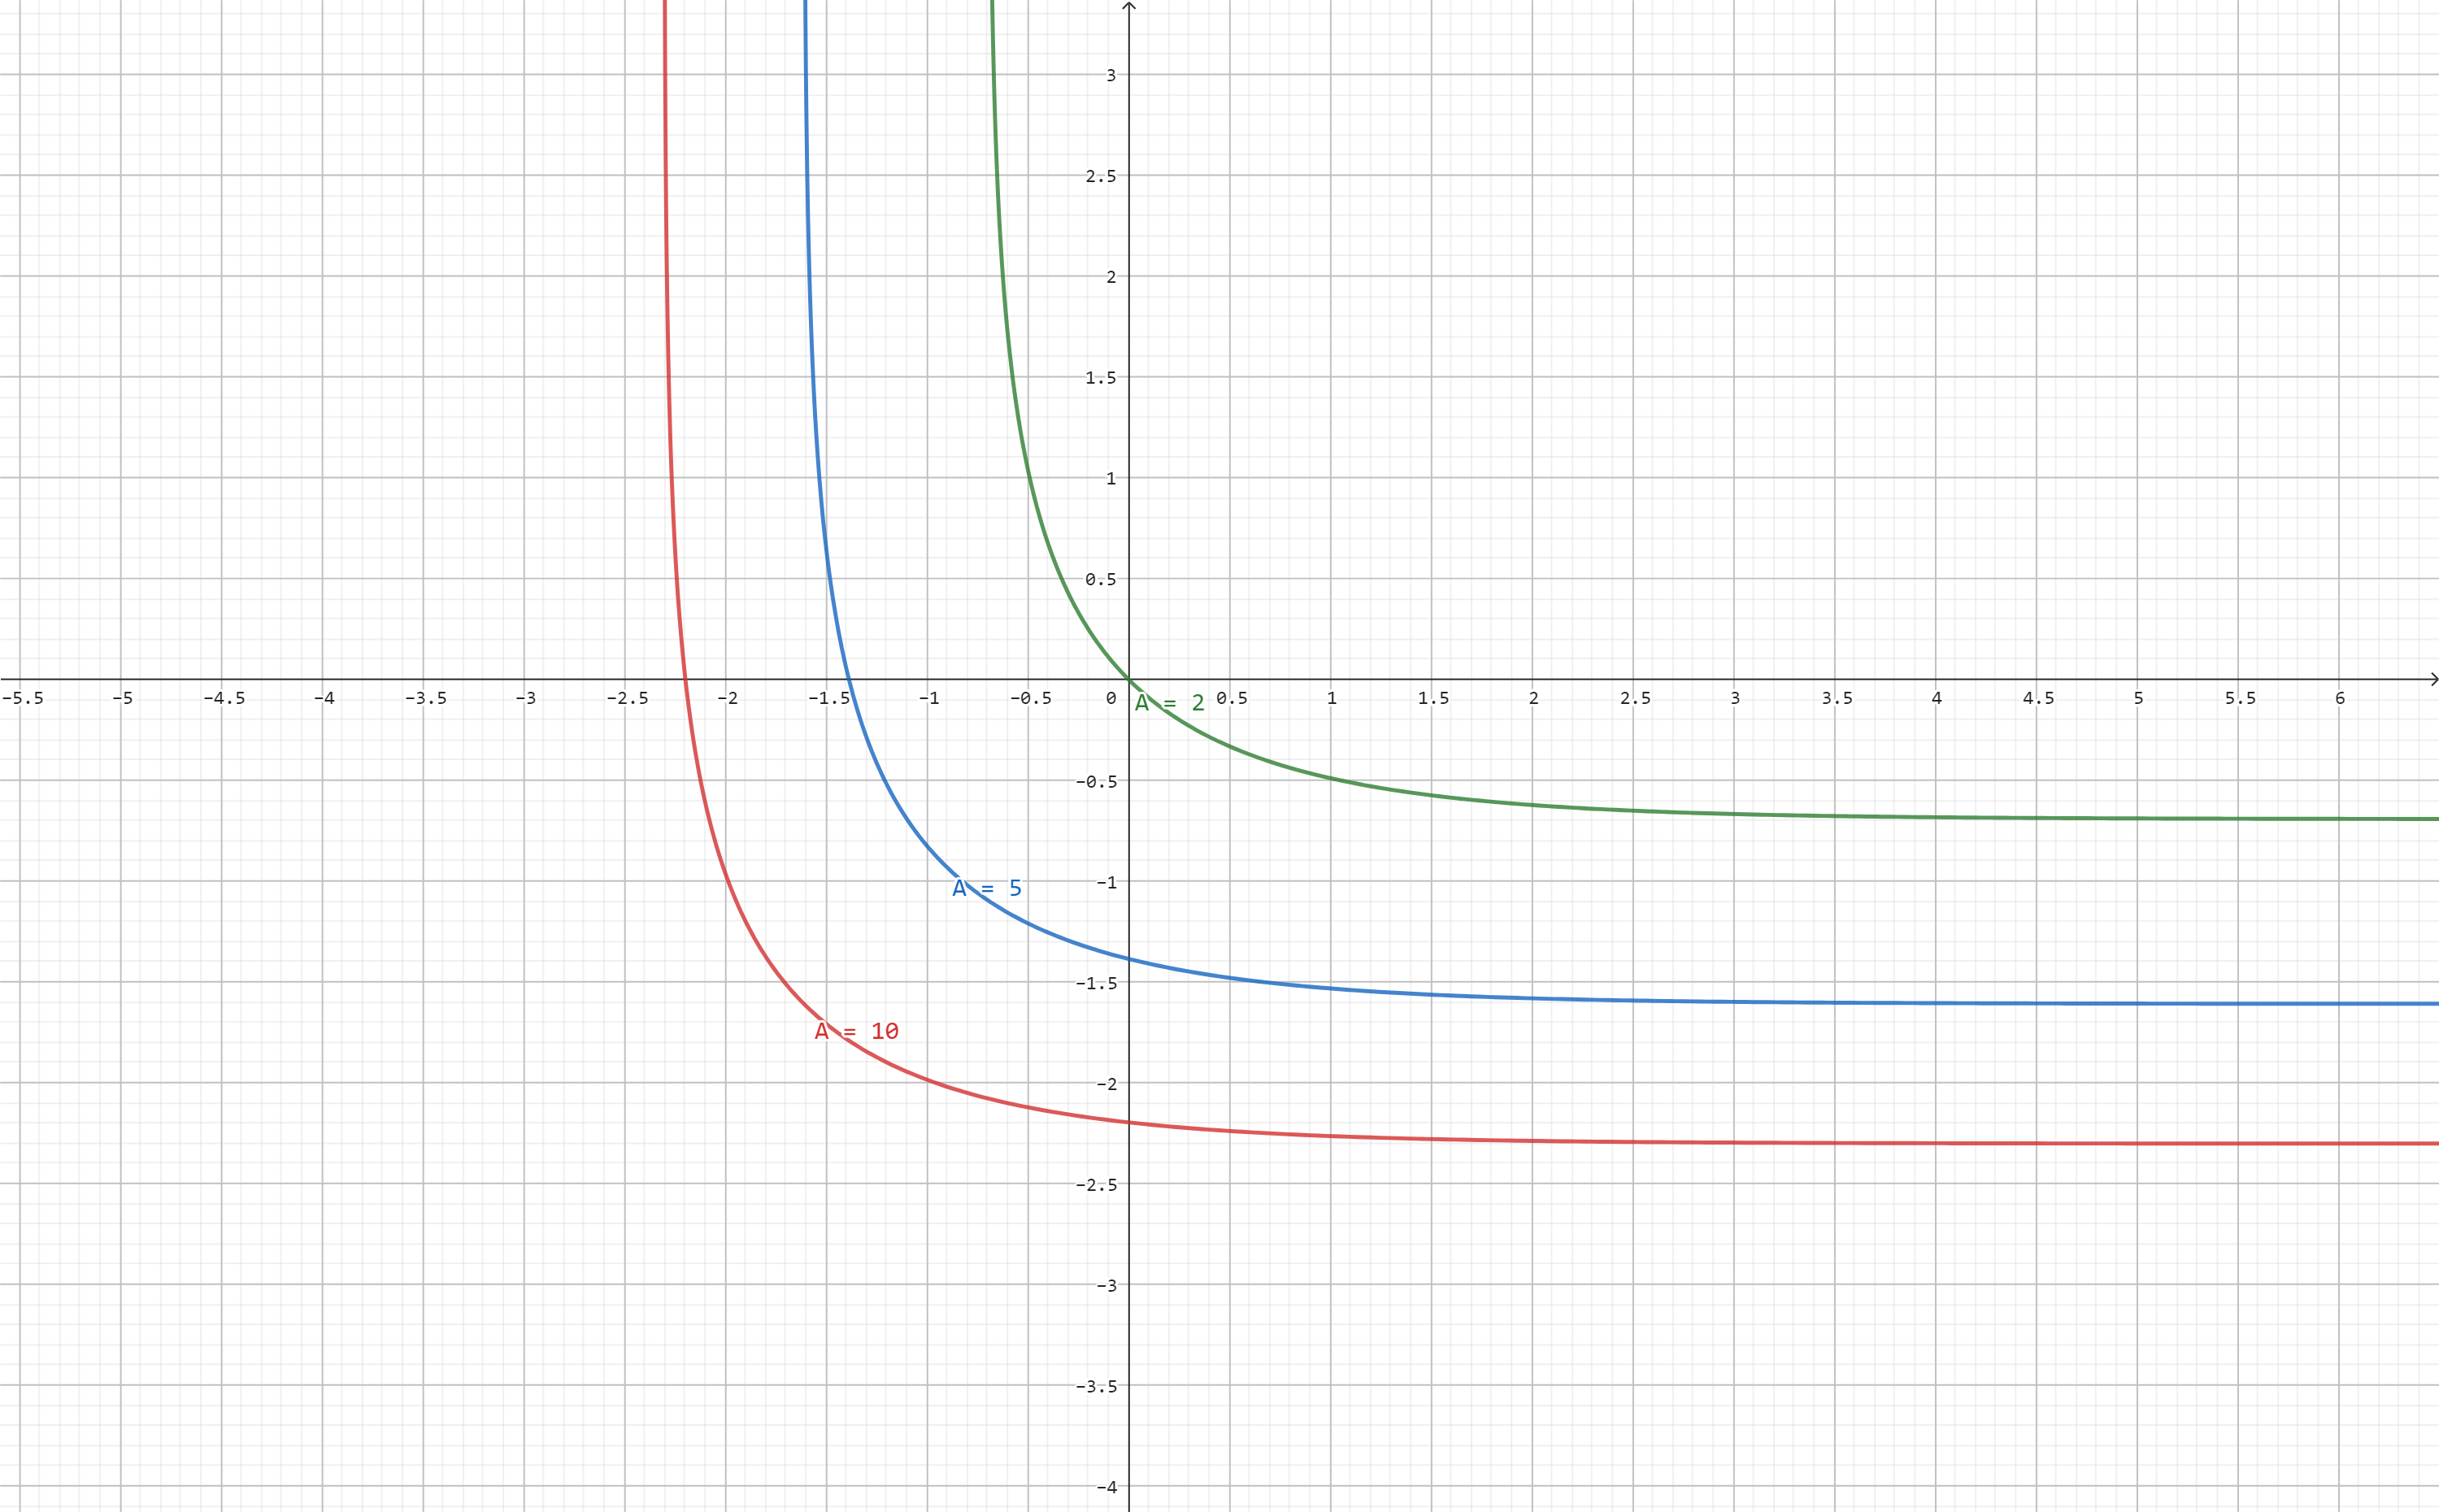
\includegraphics[width=\textwidth]{images/t02_p01.png}

\href{https://www.geogebra.org/calculator/zkyy7zap}{Ссылка на Geogebr'y}

\bigskip

Найдем потенциал \(\Phi\) поля с помощью криволинейного интеграла. Пусть точка
\(O(0, 0)\) это начало координат, а \(M(x, y)\) некоторая произвольная точка,
вычислим следующий криволинейный интеграл:

\begin{equation*}\begin{split}
    \int\limits_{OM} P(x, y)\,dx + Q(x, y)\,dy = \\
    \int\limits_{OM} e^x \,dx - e^y \,dy
  \end{split}\end{equation*}

Т.к. поле потенциально, то данный интеграл не зависит от пути и может быть
вычислен разбиением на два обычных интеграла:

\begin{equation*}\begin{split}
    \int\limits_{OM} e^x \,dx - e^y \,dy = \\
    \int_0^x e^x\,dx - \int_0^y e^y\,dy = \\
    e^x \bigg\vert_0^x - e^y \bigg\vert_0^y = \\
    e^x - 1 - e^y + 1 = \\
    e^x - e^y
  \end{split}\end{equation*}

Таким образом потенциал поля равен \(\Phi = e^x - e^y\).

\bigskip

Эквипотенциальные линии это линии, во всех точках которых потенциал имеет
одинаковое значение. Они будут задаваться уравнением \(\Phi = const\), т.е.
\(e^x - e^y = B \hspace{3pt} (B \in \mathbb{R})\).

Изобразим на графике некоторые из них при разных значениях \(B\).

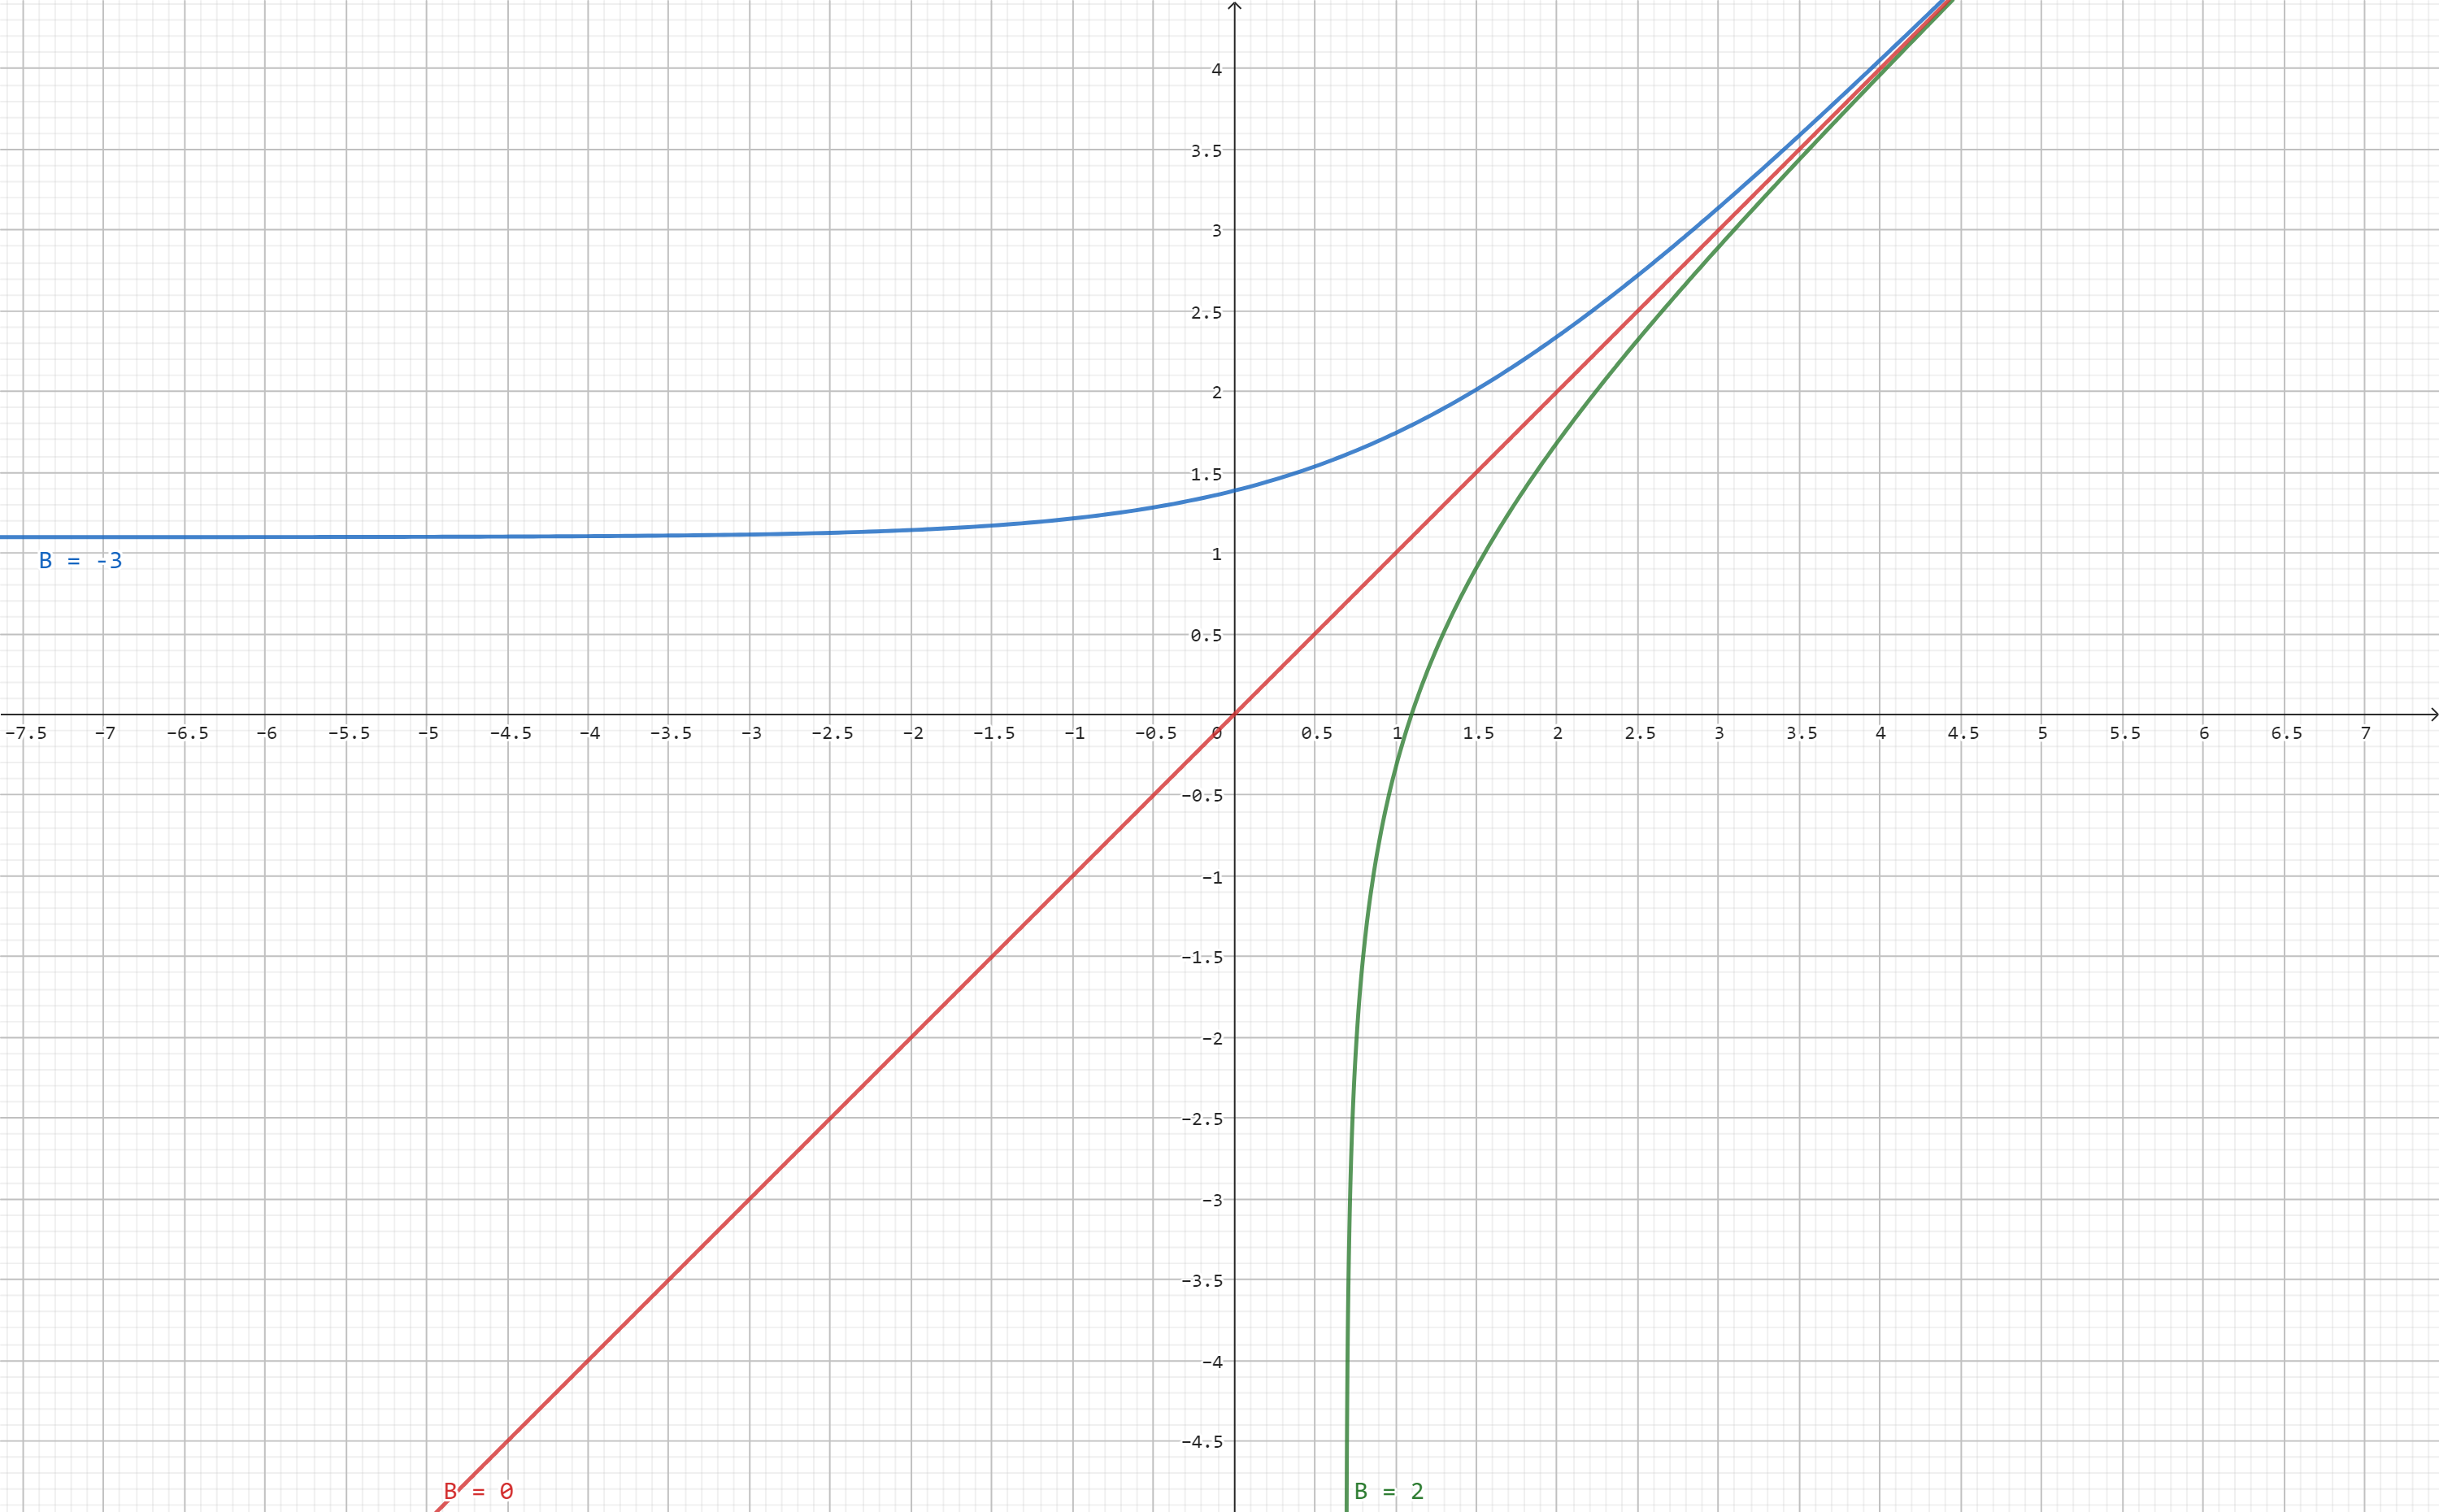
\includegraphics[width=\textwidth]{images/t02_p02.png}

\bigskip

Докажем, что эквипотенциальные линии перпендикулярны векторным линиям поля. Эти
линии будут перпендикулярны, если перпендикулярны их касательные в точке
пересечения. Обозначим точку их пересечения \((x_0, y_0)\).

Найдем наклон касательной кривой \(e^{-x} + e^{-y} - A = 0\) в этой точке.
Наклон касательной в точке равен производной в этой точке, для вычисления
производной воспользуемся формулой
\(F(x, y) = 0 \implies y' = -\dfrac{F'_x}{F'_y}\). Найдем частные производные
функции \(F(x, y)\):

\begin{equation*}\begin{split}
    F'_x = e^{-x} \cdot (-1) = -e^{-x} \\
    F'_y = e^{-y} \cdot (-1) = -e^{-y}
  \end{split}\end{equation*}

Таким образом наклон касательной к графику \(e^{-x} + e^{-y} = A\) в точке
\((x_0, y_0)\) будет равен
\(-\dfrac{e^{-x_0}}{e^{-y_0}} = -\dfrac{e^{y_0}}{e^{x_0}}\).

Аналогично найдем наклон касательной к кривой \(G(x, y) = e^x - e^y - B = 0\) в
той же точке \((x_0, y_0)\):

\begin{equation*}\begin{split}
    G'_x = e^x \\
    G'_y = -e^y
  \end{split}\end{equation*}

Таким образом наклон касательной к графику \(e^x - e^y = B\) в точке
\(x_0, y_0\) будет равен \(\dfrac{e^{x_0}}{e^{y_0}}\).

Заметим, что произведение полученных коэффициентов наклона касательных в точке
\((x_0, y_0)\) равно \(-1\). Это значит, что касательные в этой точке
перпендикулярны, а значит перпендикулярны и исходные кривые.

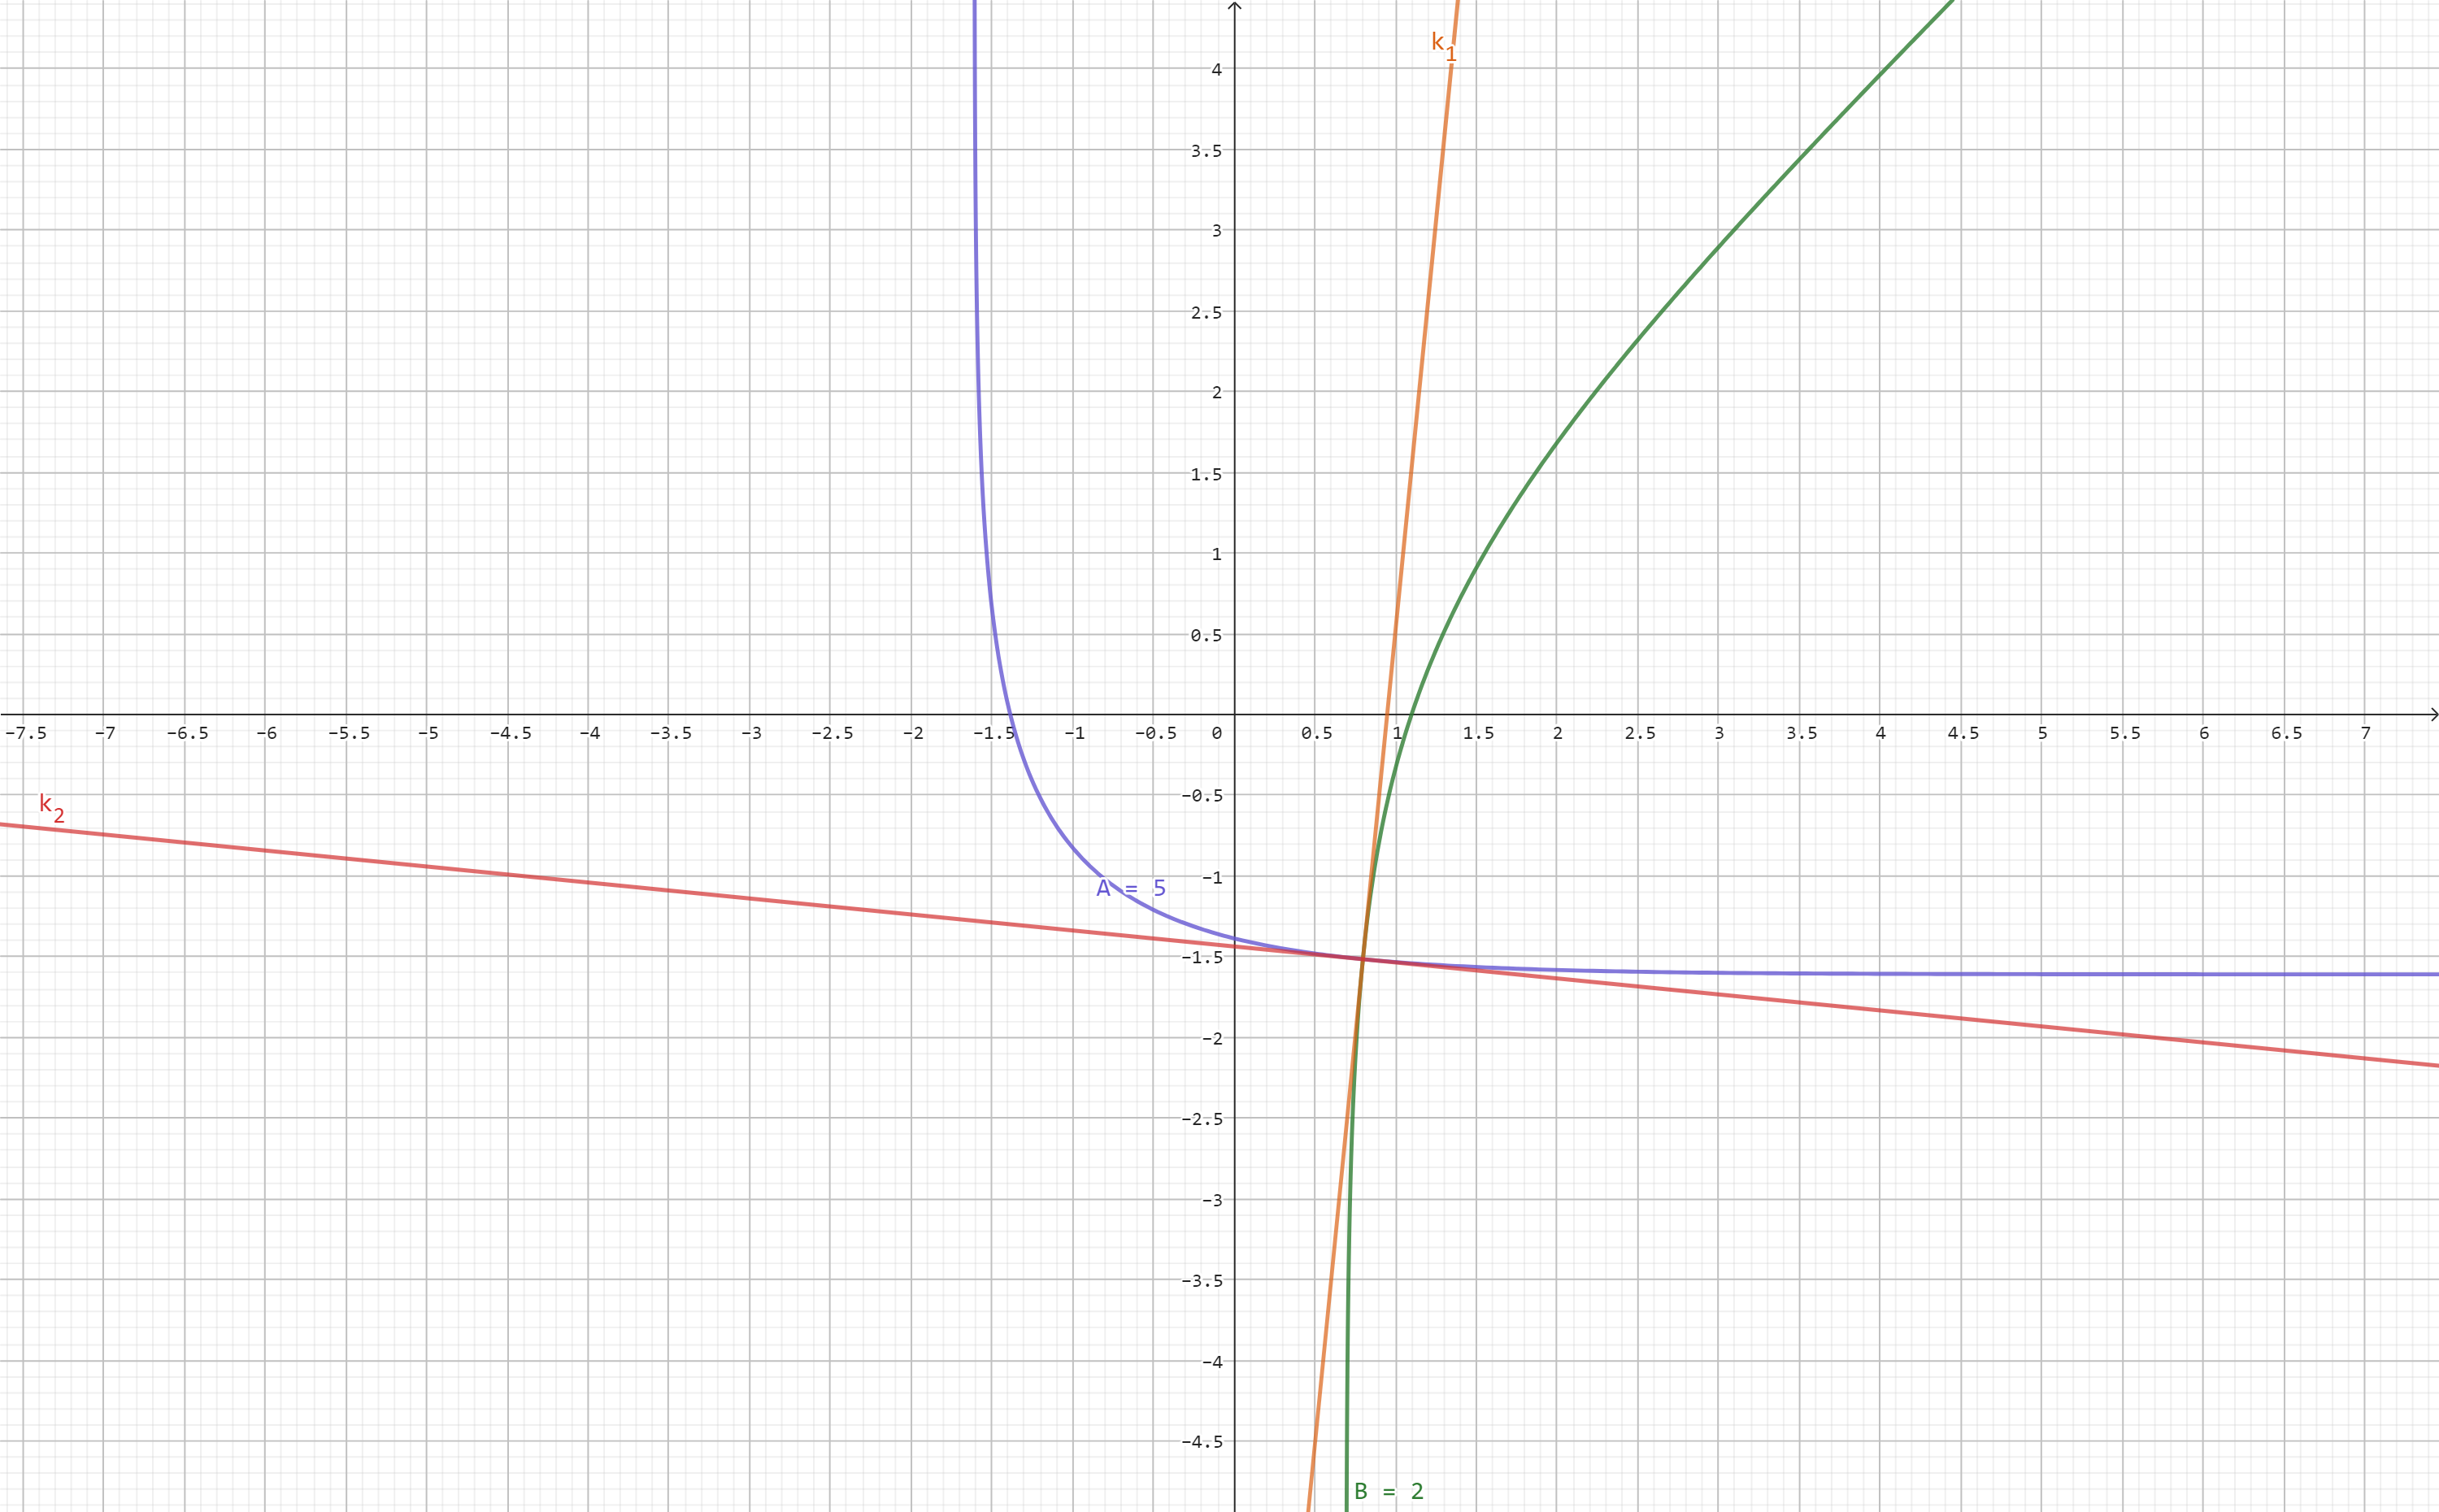
\includegraphics[width=\textwidth]{images/t02_p03.png}

\bigskip

Рассмотрим векторную линию поля \(e^{-x} + e^{-y} = e^2 + e\). Выберем две
точки, лежащие на этой линии: \(A(-2, -1)\) и \(B(-1, -2)\). Найдем работу поля
вдоль этой линии, используя найденный ранее потенциал:

\begin{equation*}\begin{split}
    W = \Phi \bigg\vert_A^B = \\
    (e^x - e^y) \bigg\vert_{(-2, -1)}^{(-1, -2)} = \\
    (e^{-1} - e^{-2}) - (e^{-2} - e^{-1}) = \\
    2e^{-1} - 2e^{-2} = \\
    \frac{2}{e^2}(e - 1)
  \end{split}\end{equation*}